\lhead{\emph{Common Classifiers}}

\chapter{Common Classifiers}
\label{common_classifiers}

The task of classification aims at categorising unknown elements to their appropriate groups. The procedure is based on quantifiable characteristics obtained from the source signal. Those characteristics, i.e.~features, are gathered in a~feature vector (a~vector of independent variables) and each pattern is described with one feature vector. It is expected that patterns accounted to the same category are in a~relationship with one another. In other words, subjects and objects of knowledge accounted to the same category are expected to be in some sense similar. There are many mathematical models that can be used as classifiers, such as SVM, random forest, kNN, regression models, or Neural Networks. Their main disadvantage lies in their need to be trained prior to usage, which makes them unable to recognize elements from a~new class, not present during the training process. This behaviour can be especially troublesome in an unstable, noisy environment, where patterns sent for classification can be corrupted, distorted or otherwise indistinguishable.

\section{Implementation}

Implementations of the common classifiers described in this chapter were taken from scikit-learn\footnote{scikit-learn webpage: \href{http://scikit-learn.org/}{http://scikit-learn.org}} Python library\cite{Pedregosa2011}. It is a popular, open source project using BSD license and built on NumPy\footnote{NumPy webpage: \href{http://www.numpy.org/}{http://www.numpy.org}}, SciPy\footnote{SciPy webpage: \href{https://www.scipy.org/}{https://www.scipy.org}} and matplotlib libraries. The project was started in 2007 by David Cournapeau as a Google Summer of Code project and is currently maintained by a team of volunteers. The library contains implementations of many algorithms to be used, among others, in classification, regression, clustering, dimensionality reduction and preprocessing problems.

\section{kNN}

The k-Nearest Neighbours algorithm, denoted as kNN, is an example of a~``lazy classifier'', where the entire training dataset is the model. There is no typical model building phase, hence the name. Class membership is determined based on class labels encountered in $k$~closest observations in the training dataset,~\cite{Altman1992}. In a~typical application, the only choice that the model designer has to make is selection of $k$~and distance metrics. Both are often determined experimentally with a~help of supervised learning procedures. Example of area coverage for three classes used in kNN classification issue can be seen in Figure \ref{fig:knn_schema}.

The kNN classifier implementation available within scikit-learn package allows to make adjustments to certain parameters that are crucial in classification issue:
\begin{itemize}
	\item $n\_neighbors$ - corresponds to the $k$ value, determines number of nearest points used to classify pattern
	\item $metric$ - the distance metric to use for the tree
\end{itemize}

\begin{figure}[htp]
	\centering
	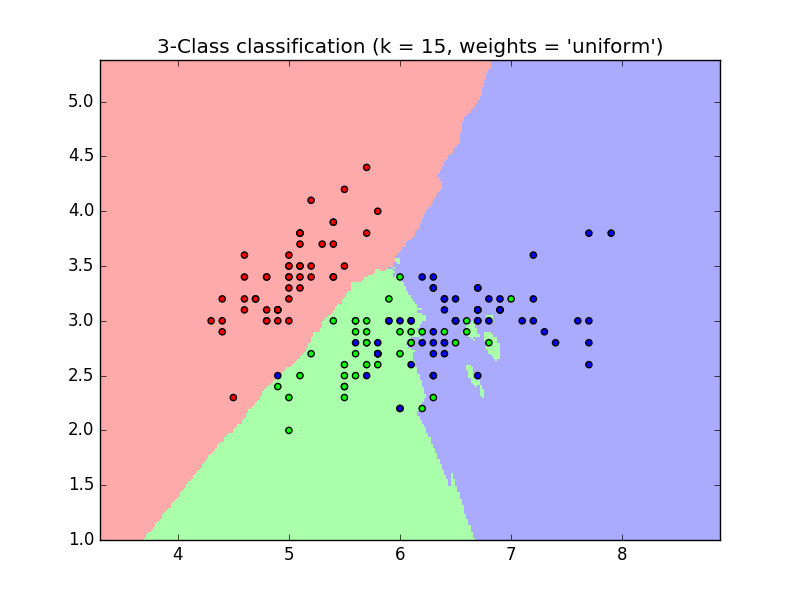
\includegraphics[width=0.7\textwidth]{Figures/knn_schema.png}
	\caption{Visualization of area coverage of three different class membership for kNN classifier with k=15, using euclidean metric. Image taken from \cite{Scikit-Learn_Website}}
	\label{fig:knn_schema}\vspace{-3pt}
\end{figure}

\section{SVM}

Support Vector Machines (SVM) are a~collection of supervised learning methods used for classification, regression and outliers detection. The SVM algorithm relies on a~construction of hyperplane with a~maximal margin that separates patterns of two classes~\cite{CortesVapnik1995}. Creation of the hyper-plane that has the largest distance to the nearest training data points of any class (so-called functional margin, can be seen on Figure \ref{fig:svm_hyperplane_margin}) is important since, in general, the larger the margin the lower the generalization error of the classifier.

\begin{figure}[htp]
	\centering
	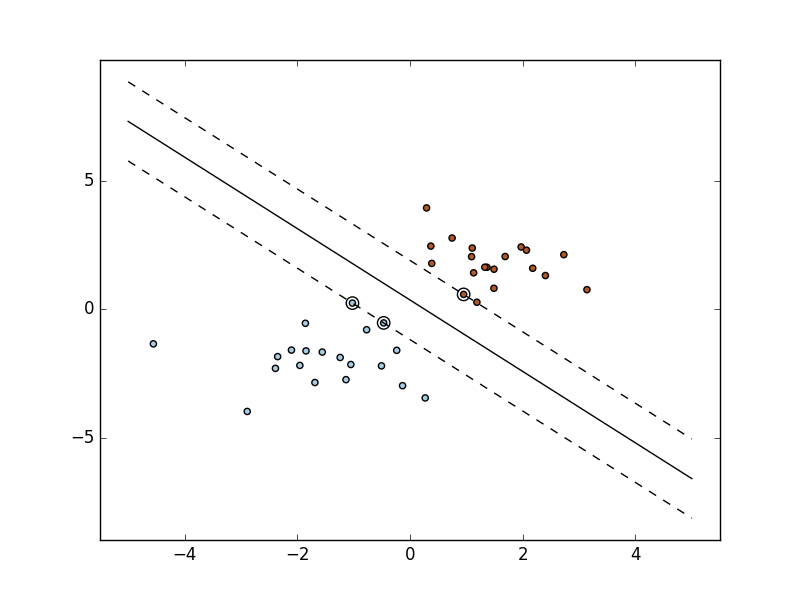
\includegraphics[width=0.7\textwidth]{Figures/svm_hyperplane_margin.png}
	\caption{SVM hyperplane construction with the biggest possible margin for training dataset. Image taken from \cite{Scikit-Learn_Website}}
	\label{fig:svm_hyperplane_margin}\vspace{-3pt}
\end{figure}

In SVM's mathematical definition the two classes' labels are denoted as -1 and 1. When treating elements from those sets as points of the Euclidean space $\mathbb{R}^{n}$ (or vectors of this space) the SVM training can be seen as the problem of finding the maximum-margin hyperplane that divides those samples. This issue can be described by formula: \[ \vec{w} * \vec{x} - b = 0 \] where $\vec{w}, \vec{x} \in \mathbb{R}^{n}, b \in \mathbb{R}$. The $\vec{x_{i}}$ vectors are samples from the training set, and $\vec{w}$ is a normal vector to the hyperplane, obtained as a linear combination of those training vectors that lie at borders of the margin: \[ \vec{w} = \Sigma_{i}\alpha_{i}\vec{x_{i}} \] Those of the training vectors $\vec{x_{i}}$ that satisfy the following condition: \[ y_{i}(\vec{x} * \vec{x_{i}} - b) = 1\] are called support vectors, and have their corresponding $\alpha_{i} \neq 0$. The $y_{i} \in \{-1, 1\}$ corresponds to the class labels that training data consists of. The linear decision function used for classifying patterns is expressed as follows: \[I(\vec{x}) = sgn(\Sigma\alpha_{i}\vec{x_{i}} * \vec{x} - b)\] where $\alpha_{i}\vec{x_{i}} = \vec{w_{i}}$. SVM efficiency can be enhanced by using different kernel functions which help in solving non-linearly-separable problems. The generalized decision function using kernel function $K$: \[I(\vec{x}) = sgn(\Sigma\alpha_{i}K(\vec{x_{i}},\vec{x}) - b)\] The sample visualization of some kernel functions can be seen on Figure \ref{fig:svm_kernel_functions}, where different class area coverages can be seen depending on the kernel function used. It's worth noting that the two higher images, although using the ``same`` linear kernel, present different results. This comes as a consequence of miscellaneous internal implementation changes that are very technical and out of scope of this paper. 

In some cases when the data is not linearly separable the hinge loss function must be introduced \[max(0, 1 - y_{i}(\vec{w}*\vec{x_{i}} - b))\] This function is zero if the $\vec{x_{i}}$ lies on the correct side of the margin. On the other hand, if the data is on the wrong side, the function's value is proportional to the distance from the margin. The aim of the SVM is to minimize the value of the hinge function for every element $\vec{x_{i}}$ from the training set.

\begin{figure}[htp]
	\centering
	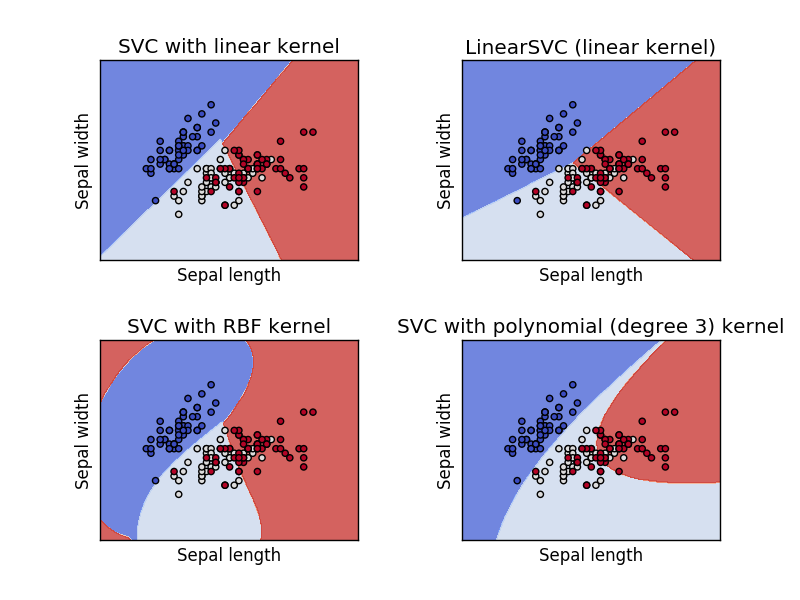
\includegraphics[width=1.0\textwidth]{Figures/svm_kernel_functions.png}
	\caption{Different class area coverages as a result of using different kernel functions. Image taken from \cite{Scikit-Learn_Website}. Please note that the two higher images show different area coverages for the ``same`` linear kernel. This difference comes from different implementations of SVC and LinearSVC classes. SVC supports multiclass classification according to one-vs-one scheme, whereas LinearSVC does it by using one-vs-rest method. According to official documentation: ``LinearSVC is implemented in terms of liblinear rather than libsvm, so it has more flexibility in the choice of penalties and loss functions and should scale better to large numbers of samples.``\cite{Scikit-Learn_Website}}
	\label{fig:svm_kernel_functions}\vspace{-3pt}
\end{figure}

SVMs are effective in high-dimensional spaces, memory efficient, and quite versatile because of the many kernel functions that can be specified for the decision function. Implementation available as part of scikit-learn package lets user specify and tweak many aspects of classifier such as:

\begin{itemize}
	\item $C$ - penalty parameter C of the error term, used to regularize the estimation. If dealing with noisy observations it's recommended to decrease its value
	\item $kernel$ - kernel type used in the algorithm, in this paper one of "poly" or "rbf" values are used. "poly" stands for polynomial kernel using following equation $(\gamma \langle x, x' \rangle + r)^{d}$ (where d is function degree, with default value 3), "rbf" is an acronym for radial basis function with given equation $exp(-\gamma|x - x'|^{2})$
	\item $gamma$ - kernel coefficient for "rbf", "poly" types as can be seen it the kernel equations
	\item $degree$ - degree of the polynomial kernel function
\end{itemize}

It is worth noting though that in some cases, where the number of features is much greater than the number of samples, using support vector machines can give poor results, and is not cost-efficient when calculating probability estimates. 

\section{Random Forest}

\begin{figure}[htp]
	\centering
	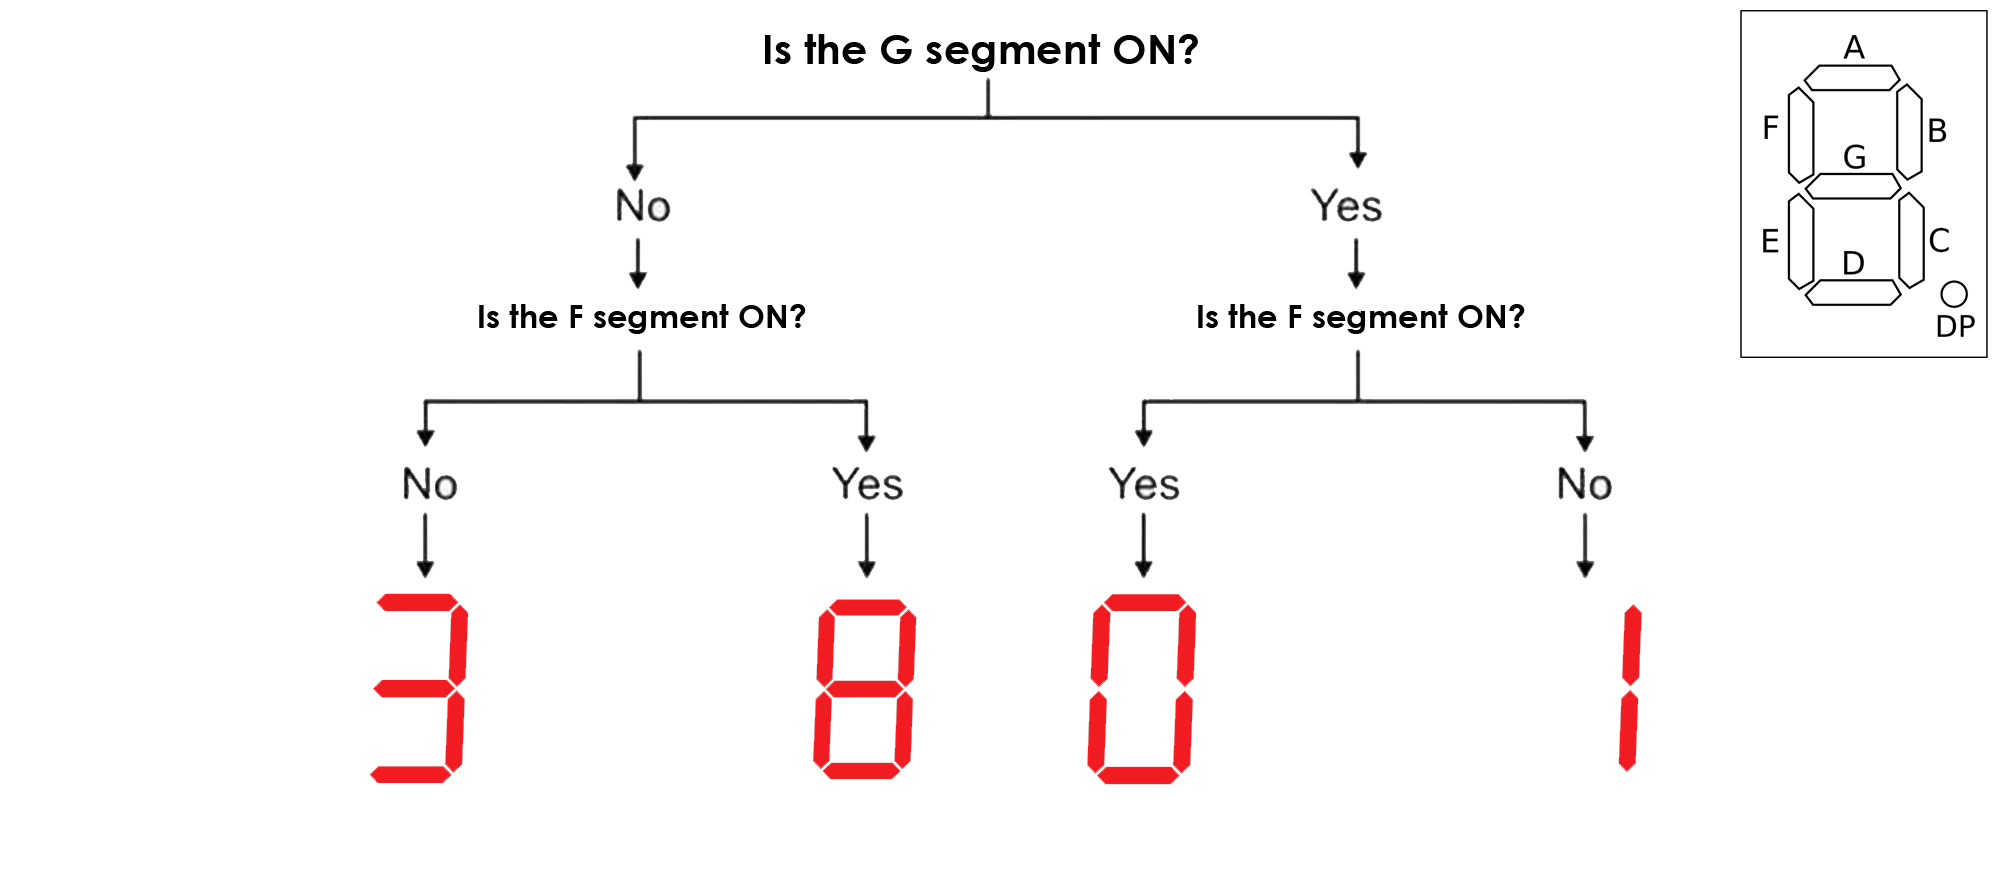
\includegraphics[width=1.0\textwidth]{Figures/rf_visualization_funny.jpg}
	\caption{An example of small decision tree}
	\label{fig:rf_visualization_funny}\vspace{-3pt}
\end{figure}

Random forest is a~popular ensemble method. The main principle behind ensemble methods, in general, is that a~group of ``weak learners'' can come together to form a~``strong learner''. In the random forest algorithm~\cite{Breiman2001} the weak learners are decision trees, which are used to predict class labels. A decision tree is a decision support tool that uses a tree-like graph for classification issue. Each graph node performs a test on an attribute of the provided pattern and sends it to its child node via a branch that represents the outcome of the test. Each leaf in a decision tree represents a certain class label. In other words for a~feature vector representing one pattern a~decision tree calculates its class label by dividing value space into two or more subspaces. More precisely, an input data is entered at the top of the tree and as it traverses down the tree the data gets bucketed into smaller subsets. There are many advantages of using decision trees. Their results are easy to interpret and visualize in form of a graph, they can handle multi class classification problems and perform well even if its assumptions are somewhat violated by the true model from which the data were generated. On the other hand, the main drawbacks connected to their usage consist of overfitting problem caused by creating too complex trees on a very complicated data, and instability caused by small variations in the data that might result in a completely different tree being generated. That last problem is easily mitigated by ensembling set of decision trees into a random forest. 

\begin{figure}[htp]
	\centering
	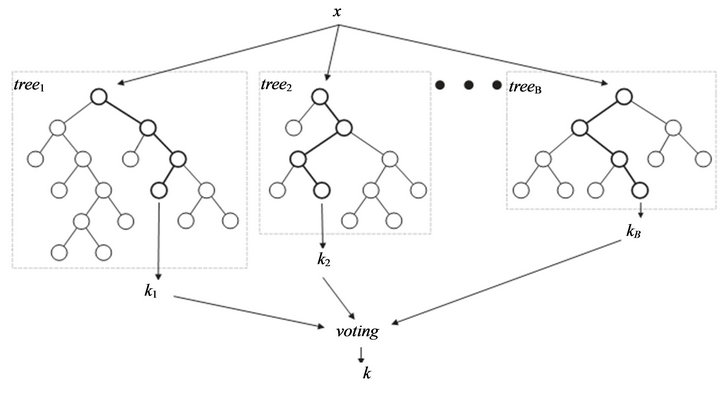
\includegraphics[width=0.85\textwidth]{Figures/rf_visualization.jpg}
	\caption{Visualization of a random forest consisting of $B$ different decision trees}
	\label{fig:rf_visualization}\vspace{-3pt}
\end{figure}

In the random forest a~large number of classification trees is formed, which altogether serve as a~classifier. In order to grow each tree, a~random selection of rows from the training set is drawn. Random sampling with replacement is also called bootstrap sampling. In addition, when constructing trees for a~random forest at each node $m$~variables out of the set of all input variables are randomly selected, and the best split on these $m$~is used to split the node. After a~relatively large number of trees is generated, they vote for the most popular class. Some of the parameters used for improving classification rates that are available within scikit-learn package random forest implementation:

\begin{itemize}
	\item $n\_estimators$ - determines number of trees used by random forest in the algorithm
	\item $max\_depth$ - the maximum depth of each tree in the forest
	\item $max\_features$ - the number of features to consider when looking for the best split
	\item $min\_samples\_leaf$ - the minimum number of samples required to be at a leaf node
\end{itemize}

Random forests join few important benefits: (a)~they are relatively prone to the influence of outliers, (b)~they have an embedded ability of feature selection, (c)~they are prone to missing values, and (d)~they are prone to over-fitting.

\section{Minimum Volume Enclosing Figures}

The easiest and probably most intuitive way of dealing with classification task is using patterns' spatial relations in order to determine their class memberships. This approach is used for example in kNN and SVM models, where point's affiliation is calculated based on its place in the features space. Every class in a dataset can be viewed as a big ``cloud`` of points and usually, if the other clouds do not overlap each other, the more dense this cloud is, the easier the task of classification gets.

Each class' cloud can be enclosed in an arbitrary geometrical shape which can be used as an identifier. The difference between binary classifiers and identifiers is very subtle, yet important. Whereas binary classifiers can distinguish between patterns from two different classes, they must be trained on data consisting of elements from both classes. Identifiers accept (or one could say: identify) only those points that they were constructed on, and reject any outliers. Thus they require only one class to be provided during training process. One of the easiest and most intuitive model of identifier is minimum volume enclosing figure. Creating figure enclosing all elements that has the smallest volume possible ensures that the identification can be very strict, which in return helps to maintain high outlier rejection rate. As opposed to convex hull, which is the most accurate point set container with smallest volume and which is enclosed by linear hyperplanes, bounding figures are far less complex. In many cases, when there is a need for computing convex hull and testing inclusions of other points, an approximation of such hull can be used, which helps in reducing time needed for computations, since most of alternative methods have lower construction and inclusion-testing complexities. Among the most popular minimum volume enclosing figures there are: boxes, diamonds, simplexes and ellipsoids.

\subsection{Minimum Volume Enclosing Ellipsoid}

\begin{figure}[htp]
	\centering
	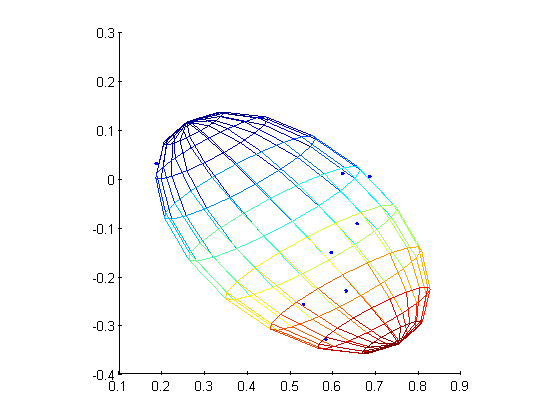
\includegraphics[width=0.70\textwidth]{Figures/minimum_bounding_ellipsoid.png}
	\caption{An example of minimum volume enclosing ellipsoid for points in 3D space}
	\label{fig:minimum_bounding_ellipsoid_visualization}\vspace{-3pt}
\end{figure}

Minimum Volume Enclosing Ellipsoid (denoted as MVEE) problem is solved by several known algorithms that can be categorized as first-order, second-order interior-point or combination of the two. For small dimensions \textit{d}, the MVEE problem can be solved in \textit{O($d^{O(d)}$m)} operations using randomized or deterministic algorithms~\cite{MVEEMichaelTodd2005}. All the results presented in this chapter were obtained while using MVEE algorithm based on Khachiyan solution.

An ellipsoid in its centre form is given by the formula:
\vspace{-6pt} 
\[ 
\vspace{-3pt}
E = \{x \in \mathbb{R}^{n} | (x - c)^{T}A(x-c) \le 1\} 
\vspace{-3pt}
\] 
where $c \in \mathbb{R}^{n}$ is the centre of the ellipse E and $ A $ is a positive definite matrix. Points lying inside the ellipsoid satisfy 
\begin{equation}(x_{i} - c)^{T}A(x_{i} - c) \le 1\end{equation} 

The technical problem that arises from using above equation comes from the inaccuracy of floating point numbers used by computers. Thus the need for providing additional variable $\varepsilon$
\begin{equation}\label{eq:ellipsoid_affiliation}(x_{i} - c)^{T}A(x_{i} - c) \le 1 + \varepsilon\end{equation} 
which defines the error margin in determining whether certain point belongs to the ellipsoid.

The main problem, when using ellipsoids as identifiers, lies in constructing them. Two main factors that decide about identification effectiveness are tolerance and acceptance parameters. Tolerance can be viewed as a threshold for ellipsoid construction accuracy (and the stop condition used in algorithm). The lower the parameter is, the more precise minimal volume ellipsoid (in terms of training point inclusion) is created. On the other hand, even with a good training set, there is a risk of not including native patterns that lie outside of the created ellipsoid (which were for example not included in the training set). Acceptance parameter (denoted as $\varepsilon$ in Equation \ref{eq:ellipsoid_affiliation}) has been introduced to prevent such unwanted behaviour. It defines a threshold for point rejection for elements lying outside of the created figure. Manipulating this parameter can be viewed as ``enlarging`` ellipsoid (by increasing $\varepsilon$ value) or ``shrinking`` it (by decreasing $\varepsilon$ value).

\subsection{Minimum Volume Enclosing Hyper Rectangle}

\begin{figure}[htp]
	\centering
	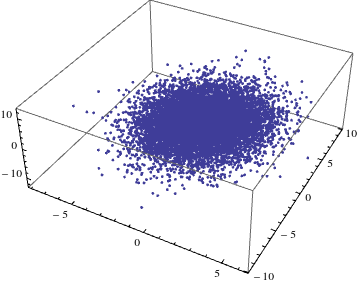
\includegraphics[width=0.40\textwidth]{Figures/minimum_bounding_box.png}
	\caption{An example of minimum bounding box for points in 3D space}
	\label{fig:minimum_bounding_box_visualization}\vspace{-3pt}
\end{figure}

Out of all possible minimum volume figures, the hyper rectangle, also called smallest enclosing box, is probably the easiest and most intuitive solution. To create such hyper rectangle one needs to store biggest and smallest values for each dimension from the training data set. Although it is straightforward to find the smallest enclosing box that has sides parallel to the coordinate axes, the difficult part of the problem is to determine the orientation of the box in the feature space. In this paper only hyper rectangles with their sides parallel to the axes are considered. The inclusion test performed for each point is done by checking whether each of the point's coordinates lies within bounds of enclosing box, and no information about the distance to the rectangle's centre is given. In case of situation when there's a need for such information the following solution, presented in form of a pseudo-code (Algorithm \ref{eq:rectangle_affiliation}) can be used.

\begin{algorithm}
	\label{eq:rectangle_affiliation}
	\caption{Algorithm for calculating point distance to hyper-rectangle centre using maximum metrics}
	\KwIn{hp - hyper-rectangle centre coordinates, p - point for which inclusion test is performed}
	\KwOut{d - distance of the point p to the hyper-rectangle centre using maximum metrics}
	d = -1 \\
	\ForEach{coordinate in hp}{
		dtmp = |p - coordinate| \\
		\If{dtmp < d}{d = dtmp}
	}
	return d \\
	\vspace{12pt}
\end{algorithm}